\documentclass[tikz,border=2pt]{standalone}

\usetikzlibrary{arrows.meta,intersections,positioning}



\begin{document}

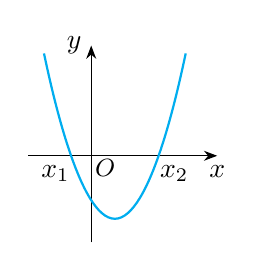
\begin{tikzpicture}[baseline={(0,0)}]
	\draw[-Stealth,name path=line](-0.8,0) -- (1.6,0)node[below]{$x$};
	\draw[-Stealth](0,-1.1) -- (0,1.4)node[left]{$y$};
	\draw[thick,cyan,name path=curve](-0.6,1.3) parabola bend(0.3,-0.8) (1.2,1.3);
	\path[name intersections={of= line and curve,name=t}]
	(t-1)node[below left= 0pt and  -3pt]{$x_1$}
	(t-2)node[below right= 0pt and  -3pt]{$x_2$};
	\node[below right=-3pt] at (0,0){\small $O$};
\end{tikzpicture}


	
\end{document}